\documentclass[tikz,border=5pt]{standalone}
\usepackage{tikz}
\usepackage{graphicx}
\pagestyle{empty}
\begin{document}
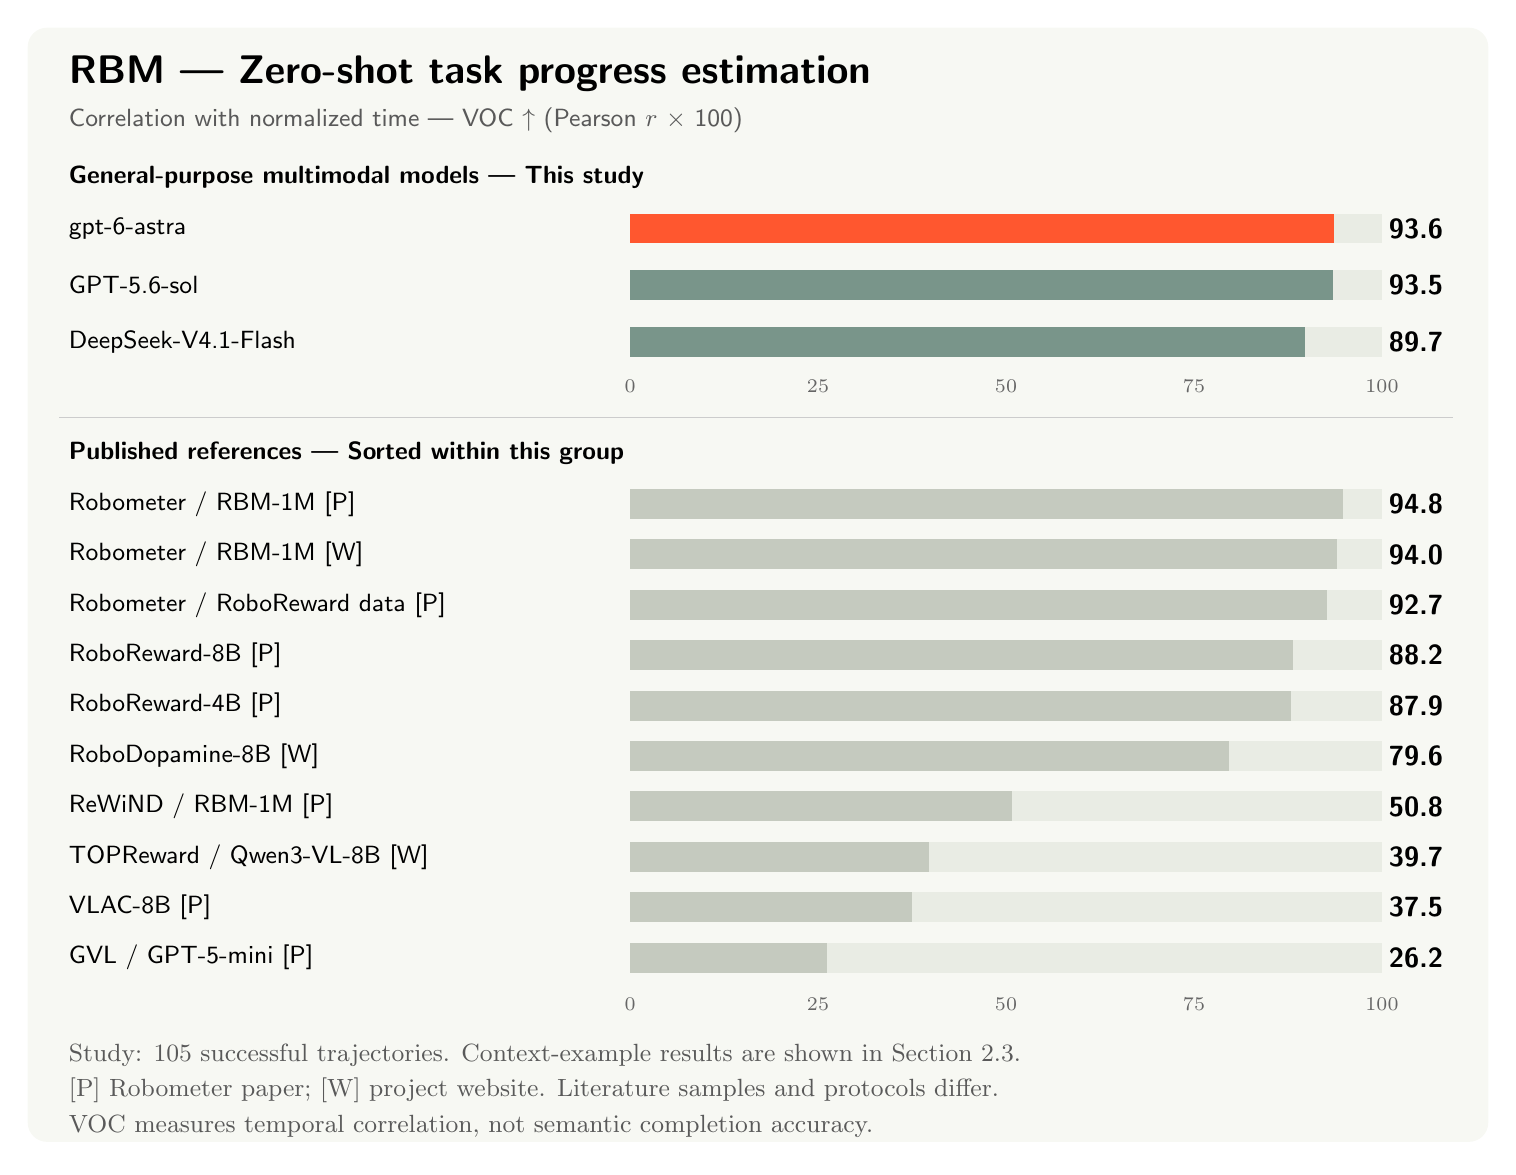
\begin{tikzpicture}[x=1cm,y=1cm,font=\sffamily]
\definecolor{cardbg}{HTML}{F7F8F3}
\definecolor{trackbg}{HTML}{E9ECE4}
\definecolor{mutedbar}{HTML}{C5CABF}
\definecolor{astrabar}{HTML}{FF572F}
\definecolor{iclbar}{HTML}{F4A082}
\definecolor{studybar}{HTML}{79958A}
\fill[cardbg,rounded corners=7pt] (-.4,2) rectangle (18.15,-12.15);
\node[anchor=west,font=\sffamily\bfseries\Large] at (0,1.42) {RBM | Zero-shot task progress estimation};
\node[anchor=west,font=\sffamily\small,text=black!65] at (0,.82) {Correlation with normalized time | VOC $\uparrow$ (Pearson $r$ $\times$ 100)};
\node[anchor=west,font=\sffamily\bfseries\small] at (0,.1) {General-purpose multimodal models | This study};
\node[anchor=west,font=\sffamily\small] at (0,-0.55) {gpt-6-astra};
\fill[trackbg] (7.25,-0.74) rectangle (16.8,-0.36);
\fill[astrabar] (7.25,-0.74) rectangle (16.188800,-0.36);
\node[anchor=east,font=\sffamily\bfseries] at (17.7,-0.55) {93.6};
\node[anchor=west,font=\sffamily\small] at (0,-1.27) {GPT-5.6-sol};
\fill[trackbg] (7.25,-1.46) rectangle (16.8,-1.08);
\fill[studybar] (7.25,-1.46) rectangle (16.179250,-1.08);
\node[anchor=east,font=\sffamily\bfseries] at (17.7,-1.27) {93.5};
\node[anchor=west,font=\sffamily\small] at (0,-1.99) {DeepSeek-V4.1-Flash};
\fill[trackbg] (7.25,-2.18) rectangle (16.8,-1.80);
\fill[studybar] (7.25,-2.18) rectangle (15.816350,-1.80);
\node[anchor=east,font=\sffamily\bfseries] at (17.7,-1.99) {89.7};
\node[text=black!60,font=\scriptsize] at (7.25,-2.55) {0};
\node[text=black!60,font=\scriptsize] at (9.6375,-2.55) {25};
\node[text=black!60,font=\scriptsize] at (12.025,-2.55) {50};
\node[text=black!60,font=\scriptsize] at (14.4125,-2.55) {75};
\node[text=black!60,font=\scriptsize] at (16.8,-2.55) {100};
\draw[black!20] (0,-2.95) -- (17.7,-2.95);
\node[anchor=west,font=\sffamily\bfseries\small] at (0,-3.4) {Published references | Sorted within this group};
\node[anchor=west,font=\sffamily\small] at (0,-4.05) {Robometer / RBM-1M [P]};
\fill[trackbg] (7.25,-4.24) rectangle (16.8,-3.86);
\fill[mutedbar] (7.25,-4.24) rectangle (16.303400,-3.86);
\node[anchor=east,font=\sffamily\bfseries] at (17.7,-4.05) {94.8};
\node[anchor=west,font=\sffamily\small] at (0,-4.69) {Robometer / RBM-1M [W]};
\fill[trackbg] (7.25,-4.88) rectangle (16.8,-4.50);
\fill[mutedbar] (7.25,-4.88) rectangle (16.227000,-4.50);
\node[anchor=east,font=\sffamily\bfseries] at (17.7,-4.69) {94.0};
\node[anchor=west,font=\sffamily\small] at (0,-5.33) {Robometer / RoboReward data [P]};
\fill[trackbg] (7.25,-5.52) rectangle (16.8,-5.14);
\fill[mutedbar] (7.25,-5.52) rectangle (16.102850,-5.14);
\node[anchor=east,font=\sffamily\bfseries] at (17.7,-5.33) {92.7};
\node[anchor=west,font=\sffamily\small] at (0,-5.97) {RoboReward-8B [P]};
\fill[trackbg] (7.25,-6.16) rectangle (16.8,-5.78);
\fill[mutedbar] (7.25,-6.16) rectangle (15.673100,-5.78);
\node[anchor=east,font=\sffamily\bfseries] at (17.7,-5.97) {88.2};
\node[anchor=west,font=\sffamily\small] at (0,-6.61) {RoboReward-4B [P]};
\fill[trackbg] (7.25,-6.80) rectangle (16.8,-6.42);
\fill[mutedbar] (7.25,-6.80) rectangle (15.644450,-6.42);
\node[anchor=east,font=\sffamily\bfseries] at (17.7,-6.61) {87.9};
\node[anchor=west,font=\sffamily\small] at (0,-7.25) {RoboDopamine-8B [W]};
\fill[trackbg] (7.25,-7.44) rectangle (16.8,-7.06);
\fill[mutedbar] (7.25,-7.44) rectangle (14.851800,-7.06);
\node[anchor=east,font=\sffamily\bfseries] at (17.7,-7.25) {79.6};
\node[anchor=west,font=\sffamily\small] at (0,-7.89) {ReWiND / RBM-1M [P]};
\fill[trackbg] (7.25,-8.08) rectangle (16.8,-7.70);
\fill[mutedbar] (7.25,-8.08) rectangle (12.101400,-7.70);
\node[anchor=east,font=\sffamily\bfseries] at (17.7,-7.89) {50.8};
\node[anchor=west,font=\sffamily\small] at (0,-8.53) {TOPReward / Qwen3-VL-8B [W]};
\fill[trackbg] (7.25,-8.72) rectangle (16.8,-8.34);
\fill[mutedbar] (7.25,-8.72) rectangle (11.041350,-8.34);
\node[anchor=east,font=\sffamily\bfseries] at (17.7,-8.53) {39.7};
\node[anchor=west,font=\sffamily\small] at (0,-9.17) {VLAC-8B [P]};
\fill[trackbg] (7.25,-9.36) rectangle (16.8,-8.98);
\fill[mutedbar] (7.25,-9.36) rectangle (10.831250,-8.98);
\node[anchor=east,font=\sffamily\bfseries] at (17.7,-9.17) {37.5};
\node[anchor=west,font=\sffamily\small] at (0,-9.81) {GVL / GPT-5-mini [P]};
\fill[trackbg] (7.25,-10.00) rectangle (16.8,-9.62);
\fill[mutedbar] (7.25,-10.00) rectangle (9.752100,-9.62);
\node[anchor=east,font=\sffamily\bfseries] at (17.7,-9.81) {26.2};
\node[text=black!60,font=\scriptsize] at (7.25,-10.4) {0};
\node[text=black!60,font=\scriptsize] at (9.6375,-10.4) {25};
\node[text=black!60,font=\scriptsize] at (12.025,-10.4) {50};
\node[text=black!60,font=\scriptsize] at (14.4125,-10.4) {75};
\node[text=black!60,font=\scriptsize] at (16.8,-10.4) {100};
\node[anchor=west,text=black!65,font=\small] at (0,-11.05) {Study: 105 successful trajectories. Context-example results are shown in Section 2.3.};
\node[anchor=west,text=black!65,font=\small] at (0,-11.5) {[P] Robometer paper; [W] project website. Literature samples and protocols differ.};
\node[anchor=west,text=black!65,font=\small] at (0,-11.95) {VOC measures temporal correlation, not semantic completion accuracy.};
\end{tikzpicture}
\end{document}
